

\tikzset{every picture/.style={line width=0.75pt}} %set default line width to 0.75pt        

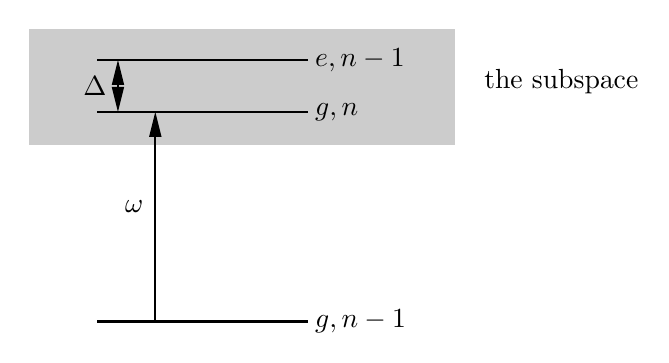
\begin{tikzpicture}[x=0.75pt,y=0.75pt,yscale=-1,xscale=1]
%uncomment if require: \path (0,300); %set diagram left start at 0, and has height of 300

%Straight Lines [id:da0992307669277781] 
\draw    (122,257.06) -- (223.5,257.06) ;
%Straight Lines [id:da7121816296099286] 
\draw    (122,156.06) -- (223.5,156.06) ;
%Straight Lines [id:da8033743672162073] 
\draw    (122,131.06) -- (223.5,131.06) ;
%Straight Lines [id:da8227639834389773] 
\draw    (150,158.06) -- (150,257.06) ;
\draw [shift={(150,156.06)}, rotate = 90] [fill={rgb, 255:red, 0; green, 0; blue, 0 }  ][line width=0.08]  [draw opacity=0] (12,-3) -- (0,0) -- (12,3) -- cycle    ;
%Straight Lines [id:da3025880663175864] 
\draw    (132,133.06) -- (132,154.06) ;
\draw [shift={(132,156.06)}, rotate = 270] [fill={rgb, 255:red, 0; green, 0; blue, 0 }  ][line width=0.08]  [draw opacity=0] (12,-3) -- (0,0) -- (12,3) -- cycle    ;
\draw [shift={(132,131.06)}, rotate = 90] [fill={rgb, 255:red, 0; green, 0; blue, 0 }  ][line width=0.08]  [draw opacity=0] (12,-3) -- (0,0) -- (12,3) -- cycle    ;
%Shape: Rectangle [id:dp7214653784779961] 
\draw  [draw opacity=0][fill={rgb, 255:red, 0; green, 0; blue, 0 }  ,fill opacity=0.2 ] (89,116) -- (294.5,116) -- (294.5,172.06) -- (89,172.06) -- cycle ;

% Text Node
\draw (225.5,257.06) node [anchor=west] [inner sep=0.75pt]    {$g,n-1$};
% Text Node
\draw (225.5,156.06) node [anchor=west] [inner sep=0.75pt]    {$g,n$};
% Text Node
\draw (225.5,131.06) node [anchor=west] [inner sep=0.75pt]    {$e,n-1$};
% Text Node
\draw (134,197.4) node [anchor=north west][inner sep=0.75pt]    {$\omega $};
% Text Node
\draw (128,143.56) node [anchor=east] [inner sep=0.75pt]    {$\Delta $};
% Text Node
\draw (307,134) node [anchor=north west][inner sep=0.75pt]   [align=left] {the subspace};


\end{tikzpicture}
